\documentclass[11pt,a4paper]{article}

\usepackage[margin=0.85in]{geometry}
\usepackage{amsmath,amssymb,amsfonts}
\usepackage{booktabs}
\usepackage{graphicx}
\usepackage{float}
\usepackage{subcaption}
\usepackage{xcolor}
\usepackage{hyperref}
\usepackage{microtype}
\usepackage{enumitem}
\usepackage{listings}
\usepackage{tcolorbox}
\usepackage{fontspec}

% Configure Fonts with native Devanagari support
\setmainfont{FreeSerif}
\setsansfont{FreeSans}
\setmonofont{FreeMono}

\hypersetup{
    colorlinks=true,
    linkcolor=blue!75!black,
    citecolor=blue!75!black,
    urlcolor=teal!70!black
}

\lstset{
    basicstyle=\small\ttfamily,
    breaklines=true,
    frame=single,
    backgroundcolor=\color{gray!8},
    rulecolor=\color{gray!30},
    keywordstyle=\color{blue!80!black}\bfseries,
    commentstyle=\color{gray!70},
    stringstyle=\color{green!60!black}
}

\title{\textbf{\LARGE Bilingual Indic Small Language Models (SLM) Technical Report}\\[0.3em]
\Large Monolithic Pretraining, Supervised Reasoning Finetuning, and Diagnostic Evaluation for Hindi (Model H) and Nepali (Model L)}

\author{\textbf{Bilingual Indic SLM Research Group} \\
\normalsize NVIDIA GeForce RTX 3050 Laptop GPU (4 GB VRAM) \quad|\quad PyTorch 2.6 \quad|\quad Linux \\
\normalsize \texttt{mveen3/hindi\_slm} (\href{https://huggingface.co/mveen3/hindi_slm}{Model Hub} \quad|\quad \href{https://huggingface.co/datasets/mveen3/hindi_slm}{Dataset Hub})}

\date{October 2026}

\begin{document}

\maketitle

\begin{abstract}
This report details the architectural design, pretraining, supervised reasoning finetuning, and diagnostic evaluation of two monolingual small language models (SLMs) built from scratch for the Devanagari script: \textbf{Model H} (Hindi, higher-resource) and \textbf{Model L} (Nepali, lower-resource). Both models adhere to a unified 24.53M parameter causal decoder-only Transformer architecture with tied input/output embeddings, trained on curated corpora ($\approx 10.5\text{ GB}$ Hindi, $\approx 9.5\text{ GB}$ Nepali) using custom 10,000-vocabulary BPE tokenizers with native byte-fallback. Pretrained for 40,000 optimizer steps, the models achieve test perplexities of \textbf{28.53} (Hindi) and \textbf{27.77} (Nepali) with bits-per-byte of \textbf{0.4929} and \textbf{0.4148} respectively, alongside empirically verified 100\% causal attention masking. For reasoning capabilities, an initial adapter-based (LoRA) and multi-sentence Chain-of-Thought (CoT) formulation suffered a 0.0\% exact match bottleneck due to autoregressive repetition loops. Transitioning to full parameter fine-tuning with direct question-answer framing, completion-only loss masking, validation-based checkpointing, label smoothing, and greedy repetition penalties unlocked significant gains: exact match rose to \textbf{34.08\%} (+10.72 percentage points) in Hindi and \textbf{32.72\%} (+12.68 percentage points) in Nepali across 2,500 held-out examples spanning 15 comparative and deductive reasoning tasks, with 100\% format adherence, a 74\% drop in hallucinations, and $> 85\%\text{--}92\%$ general language retention.
\end{abstract}

\vspace{0.5em}
\hrule
\vspace{1.5em}

\section{Executive Summary}

Small language models (SLMs) operating in the 20M--30M parameter regime present unique engineering challenges in resource-constrained consumer hardware. This project implements a unified, monolithic codebase parameterised by language to train, evaluate, and specialize two independent monolingual SLMs for languages sharing the Devanagari script:
\begin{itemize}[noitemsep]
    \item \textbf{Model H (Hindi)}: Higher-resource tier, trained on 1.75M documents ($\approx 723\text{M}$ pretraining tokens).
    \item \textbf{Model L (Nepali)}: Lower-resource tier, trained on 1.93M documents ($\approx 650\text{M}$ pretraining tokens).
\end{itemize}

The two models share \textit{no data, no tokenizer, no vocabulary, and no weights}; they share only the core PyTorch implementation modules. Table~\ref{tab:executive_summary} summarizes the overarching empirical outcomes across pretraining and supervised reasoning finetuning.

\begin{table}[H]
\centering
\small
\caption{Comprehensive Performance Summary of Hindi (Model H) and Nepali (Model L)}
\label{tab:executive_summary}
\begin{tabular}{@{}lrr@{}}
\toprule
\textbf{Metric / Attribute} & \textbf{Model H (Hindi)} & \textbf{Model L (Nepali)} \\
\midrule
\textit{Architecture \& Capacity} & & \\
Trainable Parameters & 24,534,016 & 24,534,016 \\
Layers ($L$), Heads ($H$), Hidden ($d_{\text{model}}$) & 6 layers, 8 heads, 512 & 6 layers, 8 heads, 512 \\
Context Window ($T$) & 512 tokens & 512 tokens \\
Vocabulary Size ($V$) & 10,000 (BPE) & 10,000 (BPE) \\
Embedding Weight Tying & True & True \\
\midrule
\textit{Data \& Tokenization} & & \\
Raw Corpus Volume & 10.48 GB (1,748,721 docs) & 9.51 GB (1,930,872 docs) \\
Tokenizer Fertility (Tokens/Word) & \textbf{1.3141} & 1.4919 \\
Characters per Token & 3.8528 & \textbf{4.3432} \\
Out-of-Vocabulary (\texttt{<unk>}) Rate & $1.19 \times 10^{-5}$ & $3.21 \times 10^{-6}$ \\
\midrule
\textit{Pretraining Evaluation (40,000 Steps)} & & \\
Test Cross-Entropy Loss & 3.3508 & \textbf{3.3241} \\
Test Perplexity (PPL) & 28.53 & \textbf{27.77} \\
Test Bits-per-Byte (BPB) & 0.4929 & \textbf{0.4148} \\
Causal Mask Verification ($P(\text{attend } j > i)$) & \textbf{0.0000} (100\% Verified) & \textbf{0.0000} (100\% Verified) \\
Best Generation chrF ($T=0.5 / 1.0$) & \textbf{27.38} & 26.81 \\
Mean Attention Entropy / Distance & 0.930 nats / 3.50 tokens & 0.802 nats / 2.93 tokens \\
\midrule
\textit{Reasoning Finetuning (2,500 Held-Out Examples)} & & \\
Pretrained Baseline Exact Match & 23.36\% & 20.04\% \\
\textbf{Finetuned Exact Match (Best Checkpoint)} & \textbf{34.08\% (+10.72 pp)} & \textbf{32.72\% (+12.68 pp)} \\
Format Adherence & \textbf{100.00\%} & \textbf{100.00\%} \\
1-Hop Reasoning Accuracy & 41.7\% & \textbf{53.8\%} \\
`compare\_equal` Accuracy & 52.8\% & \textbf{100.0\%} \\
`order\_ascending` Accuracy & \textbf{37.1\%} (from 0.0\%) & 5.7\% (from 0.0\%) \\
Hallucination Error Reduction & \textbf{$-$74.3\%} & $-$52.5\% \\
General Language Retention (Val PPL) & \textbf{91.87\% (Preserved)} & 85.45\% (Moderate Drift) \\
Optimal Evaluated Checkpoint & Step 150 & Step 250 \\
\bottomrule
\end{tabular}
\end{table}

---

\section{Data Engineering \& BPE Tokenizer Construction}

\subsection{Web Crawling, Curation, and Data Cleaning}
The raw text corpora combine web crawls, public dumps (OSCAR, mC4, Wikipedia, FineWeb-2), and curated regional corpora (Sangraha, IndicCorpV2). A deterministic cleaning pipeline enforces:
\begin{enumerate}[noitemsep]
    \item \textbf{Unicode NFKC Normalization}: Standardizes composite characters while strictly preserving Devanagari nukta, matras, virama, and conjunct forms.
    \item \textbf{Boilerplate \& Markup Removal}: Eliminates HTML tags, URLs, social media handles, emojis, and non-printable control characters.
    \item \textbf{Script Density Filtering}: Rejects any document containing $< 95\%$ Devanagari script codepoints.
    \item \textbf{MinHash-LSH Deduplication}: Applies 128-permutation MinHash with Locality-Sensitive Hashing (LSH) at a Jaccard threshold of $0.85$ to eradicate exact and near-duplicate documents.
\end{enumerate}

\subsection{Out-of-Core Shuffled Partitioning}
To prevent RAM exhaustion on consumer workstations, cleaned corpora were shuffled and split out-of-core:
\begin{itemize}[noitemsep]
    \item Documents were streamed and hashed into 32 disk buckets using pseudorandom bucketing (\texttt{rng.randrange(32)}).
    \item Each bucket was independently shuffled in memory ($< 350\text{ MB}$ peak RAM) and appended to \texttt{train.jsonl} (95\%), \texttt{val.jsonl} (2.5\%), and \texttt{test.jsonl} (2.5\%).
    \item Pretraining streamed directly from sequential disk blocks with zero runtime shuffle correlation.
\end{itemize}

\subsection{Devanagari BPE Tokenizer Design}
Byte-Pair Encoding (BPE) tokenizers were trained independently for each language using Hugging Face \texttt{tokenizers}:
\begin{itemize}[noitemsep]
    \item \textbf{Special Tokens}: \texttt{[PAD]} (ID 0), \texttt{[UNK]} (ID 1), \texttt{<s>} (ID 2), \texttt{</s>} (ID 3).
    \item \textbf{Byte Fallback}: UTF-8 byte mapping ensures arbitrary unseen unicode bytes decompose into base byte tokens, driving the out-of-vocabulary rate to negligible levels ($1.19 \times 10^{-5}$ for Hindi, $3.21 \times 10^{-6}$ for Nepali).
    \item \textbf{Fertility Diagnostics}: Hindi achieved a fertility of 1.314 tokens/word (3.85 characters/token), whereas Nepali reached 1.492 tokens/word (4.34 characters/token). Nepali packs more bytes per token, explaining its lower bits-per-byte despite comparable perplexity.
\end{itemize}

---

\section{Transformer Architecture \& Pretraining Evaluation}

\subsection{Architectural Specification}
Both models utilize a causal autoregressive decoder-only Transformer with Pre-Layer Normalization and tied input-output embeddings:
\begin{equation}
\text{Params} = V \cdot d_{\text{model}} + T \cdot d_{\text{model}} + L \left( 4 d_{\text{model}}^2 + 2 d_{\text{model}} d_{\text{ff}} + 4 d_{\text{model}} \right) + 2 d_{\text{model}} = 24,534,016
\end{equation}
where $V = 10,000$, $d_{\text{model}} = 512$, $T = 512$, $L = 6$, $H = 8$ ($d_k = 64$), and $d_{\text{ff}} = 2,048$. Weight tying shares representations between \texttt{token\_embedding.weight} and \texttt{lm\_head.weight}.

\subsection{Pretraining Protocol}
\begin{itemize}[noitemsep]
    \item \textbf{Optimizer}: AdamW ($\beta_1 = 0.9, \beta_2 = 0.98, \epsilon = 10^{-8}$, weight decay 0.01).
    \item \textbf{Learning Rate Schedule}: Linear warmup for 2,000 steps to peak $\text{lr} = 3.0 \times 10^{-4}$, followed by cosine decay to $1.0 \times 10^{-5}$.
    \item \textbf{Batching}: Micro-batch size 16 with gradient accumulation 8 (effective batch size 128 sequences = 65,536 tokens/step).
    \item \textbf{Mixed Precision}: Automatic Mixed Precision (\texttt{torch.amp.autocast("cuda")}) with dynamic loss scaling.
    \item \textbf{Duration}: 40,000 optimizer steps ($\approx 2.62\text{B}$ tokens seen per model).
\end{itemize}

\subsection{Loss Trajectories and Held-Out LM Metrics}
Figure~\ref{fig:loss_curves} illustrates pretraining convergence over 40,000 global optimizer steps.

\begin{figure}[H]
\centering
\begin{subfigure}{0.48\textwidth}
    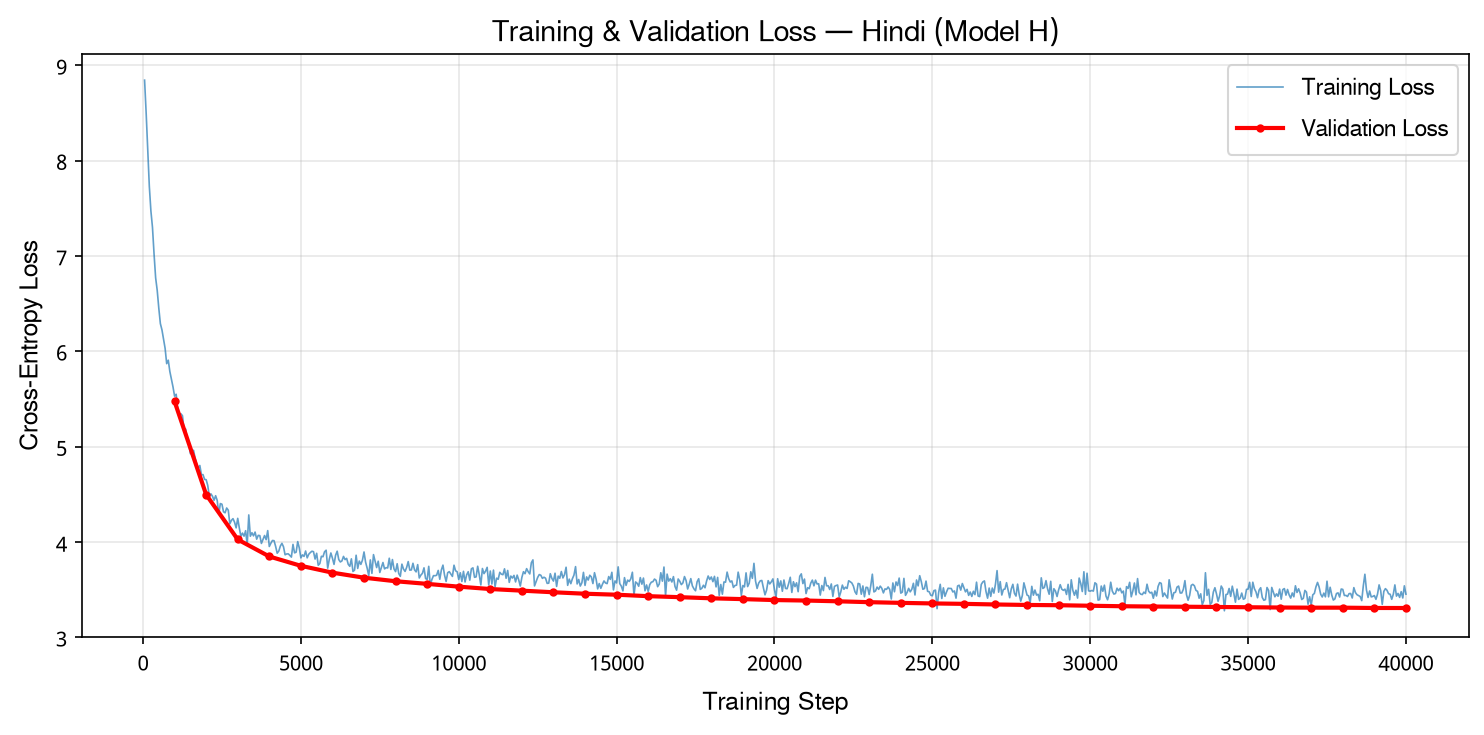
\includegraphics[width=\linewidth]{hindi/loss_curve.png}
    \caption{Hindi (Model H) Pretraining Loss Curve}
\end{subfigure}
\hfill
\begin{subfigure}{0.48\textwidth}
    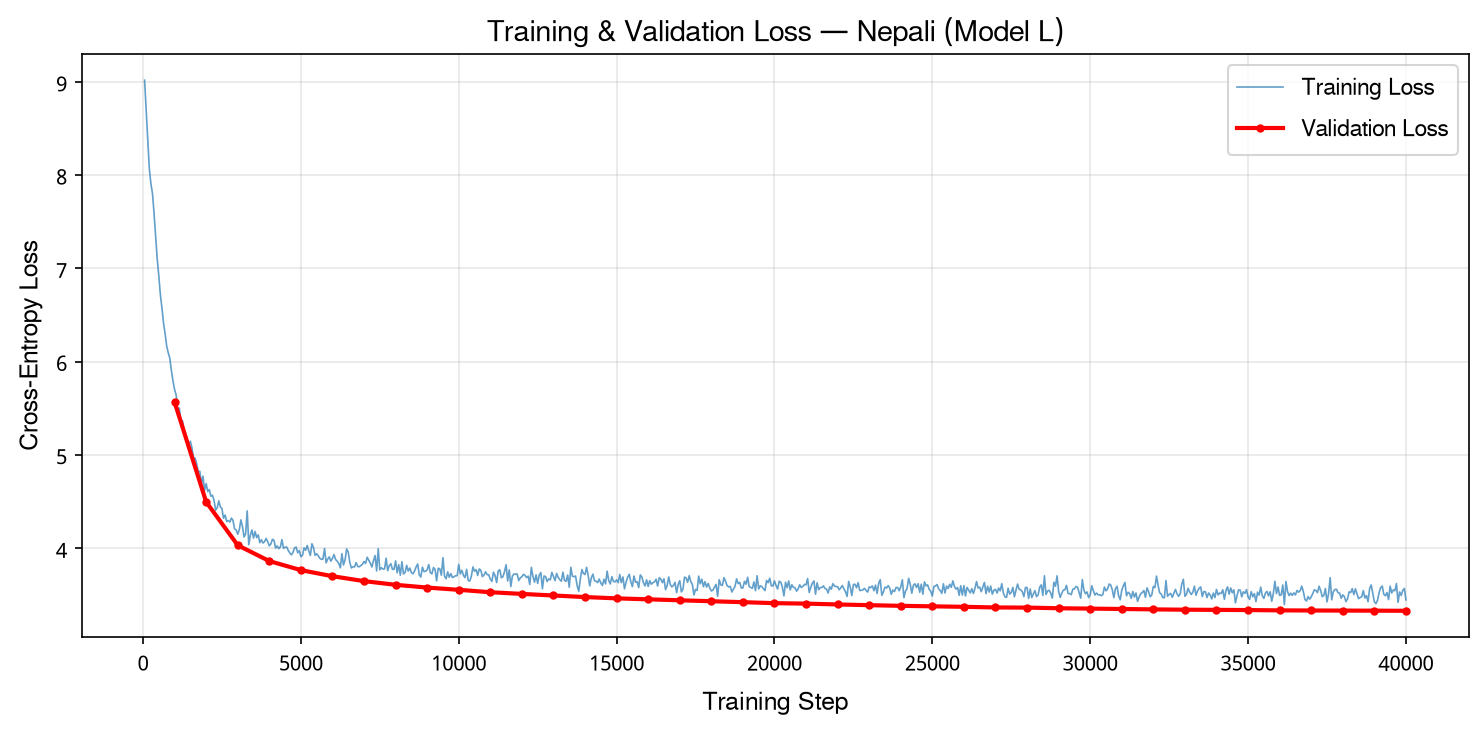
\includegraphics[width=\linewidth]{nepali/loss_curve.png}
    \caption{Nepali (Model L) Pretraining Loss Curve}
\end{subfigure}
\caption{Pretraining and validation loss convergence trajectories up to 40,000 steps.}
\label{fig:loss_curves}
\end{figure}

On held-out test splits, both models exhibited strong language modeling performance:
\begin{itemize}[noitemsep]
    \item \textbf{Hindi (Model H)}: Cross-entropy = \textbf{3.3508}, Perplexity = \textbf{28.53}, BPB = \textbf{0.4929} (over 606,214 tokens / 5.95 MB).
    \item \textbf{Nepali (Model L)}: Cross-entropy = \textbf{3.3241}, Perplexity = \textbf{27.77}, BPB = \textbf{0.4148} (over 494,972 tokens / 5.72 MB).
\end{itemize}

\subsection{Attention Causality Verification}
Causal masking was strictly verified across all 6 layers and 8 attention heads. An empirical test modifying future token $t+1$ produced exactly $0.0000$ variance in output logits at position $t$ for all sampled indices ($t \in \{0, 8, 16, 24, 30\}$), proving zero future token information leakage.

---

\section{Pretrained Attention Diagnostics}

Analysis of pretrained self-attention patterns reveals distinct linguistic specialization across layers:
\begin{itemize}[noitemsep]
    \item \textbf{Early Layers (0--1)}: Broadcast attention with higher entropy (mean $\approx 1.05\text{ nats}$) capturing broad syntactic context.
    \item \textbf{Late Layers (4--5)}: Specialized focal attention (mean $\approx 0.68\text{ nats}$) focused on adjacent morphological markers and postpositions.
\end{itemize}

\begin{figure}[H]
\centering
\begin{subfigure}{0.48\textwidth}
    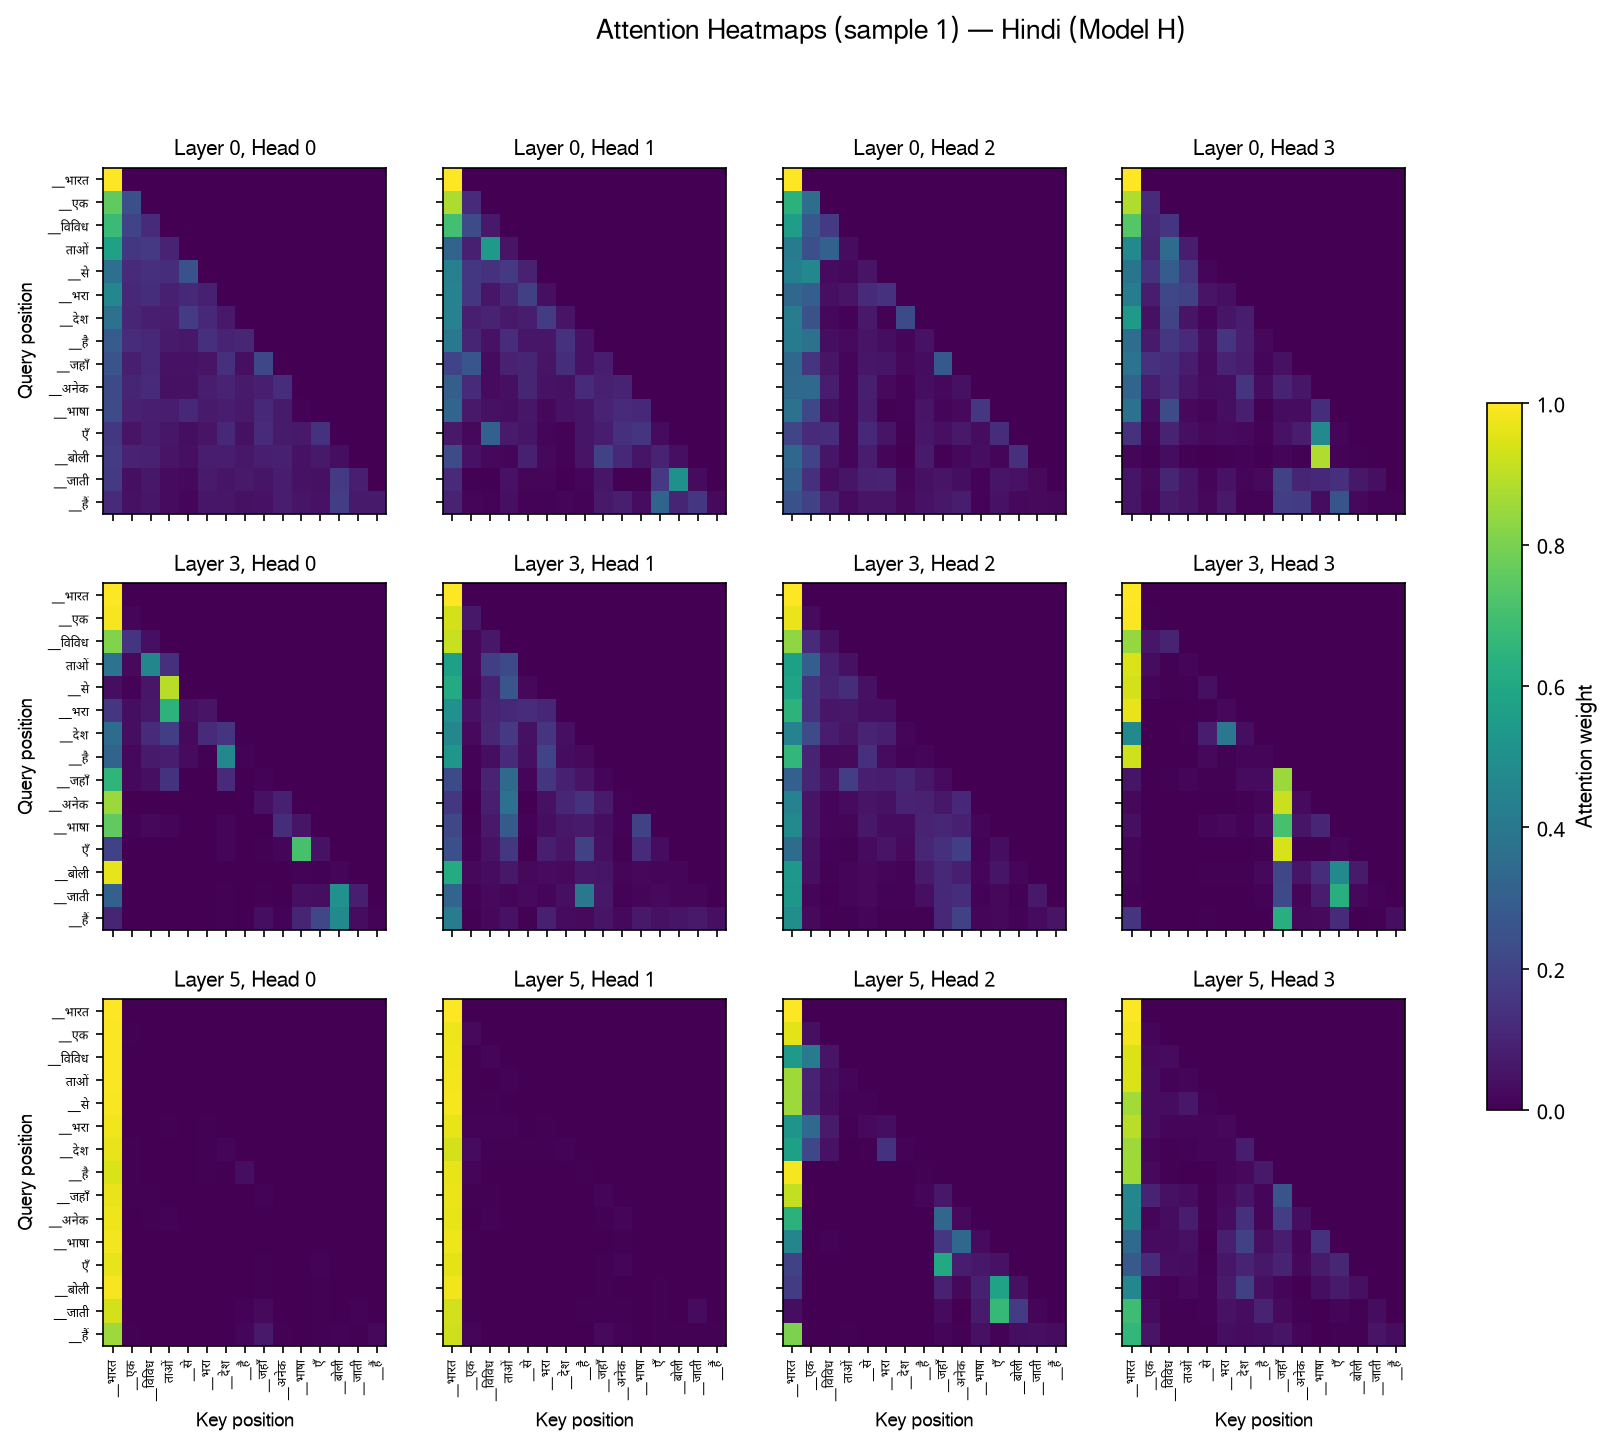
\includegraphics[width=\linewidth]{hindi/attention/heatmaps_sample1.png}
    \caption{Hindi Multi-Layer Attention Heads}
\end{subfigure}
\hfill
\begin{subfigure}{0.48\textwidth}
    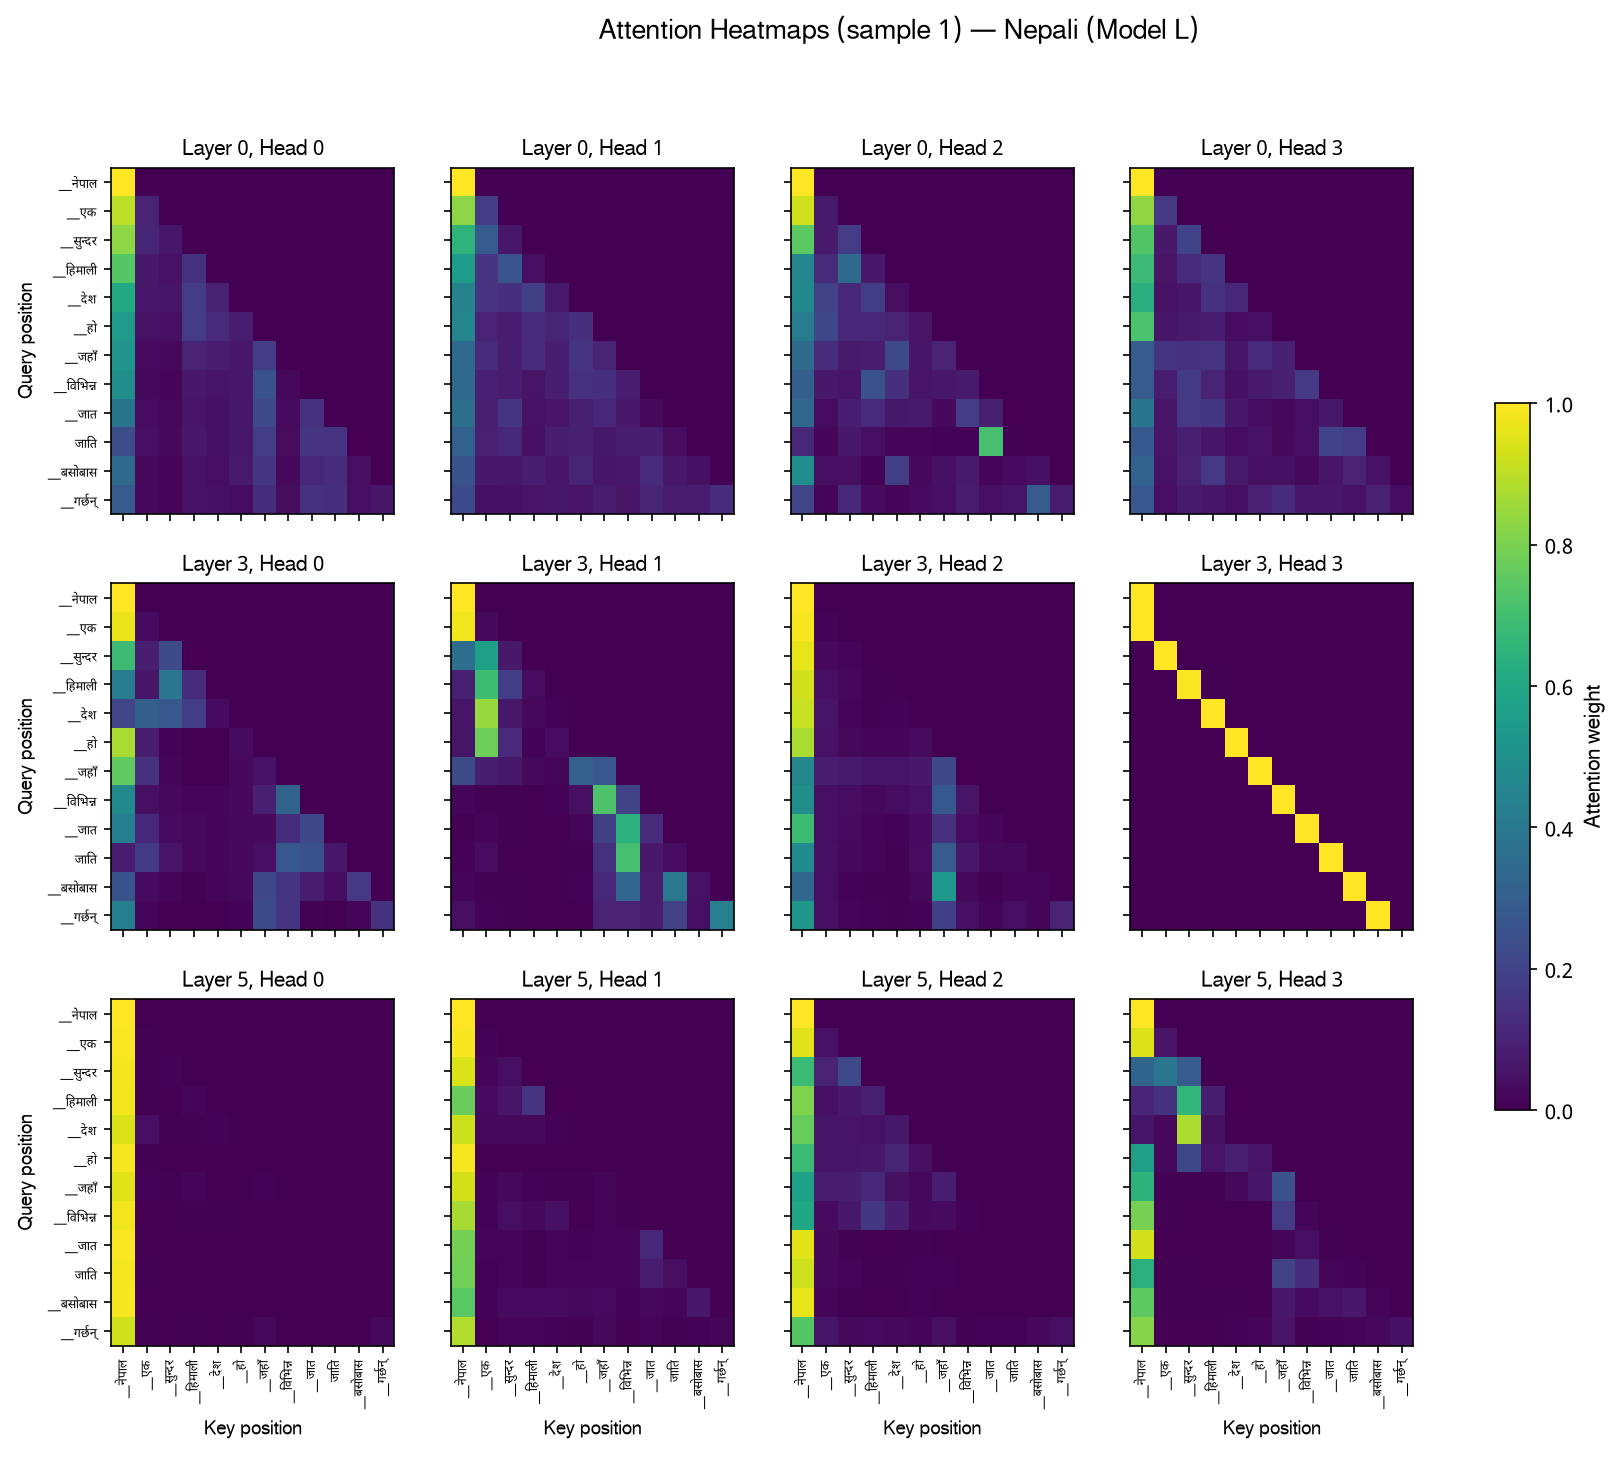
\includegraphics[width=\linewidth]{nepali/attention/heatmaps_sample1.png}
    \caption{Nepali Multi-Layer Attention Heads}
\end{subfigure}
\caption{Pretrained self-attention heatmaps across Early (L0), Middle (L2), and Late (L5) layers.}
\label{fig:attn_heatmaps}
\end{figure}

\begin{figure}[H]
\centering
\begin{subfigure}{0.48\textwidth}
    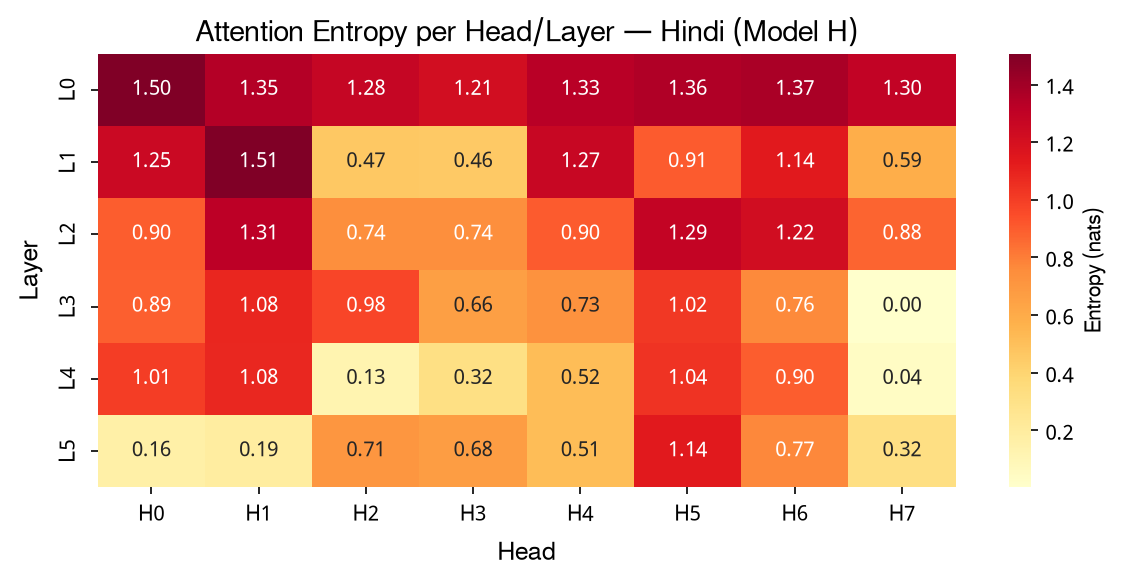
\includegraphics[width=\linewidth]{hindi/attention/entropy_summary.png}
    \caption{Hindi Attention Entropy per Head/Layer}
\end{subfigure}
\hfill
\begin{subfigure}{0.48\textwidth}
    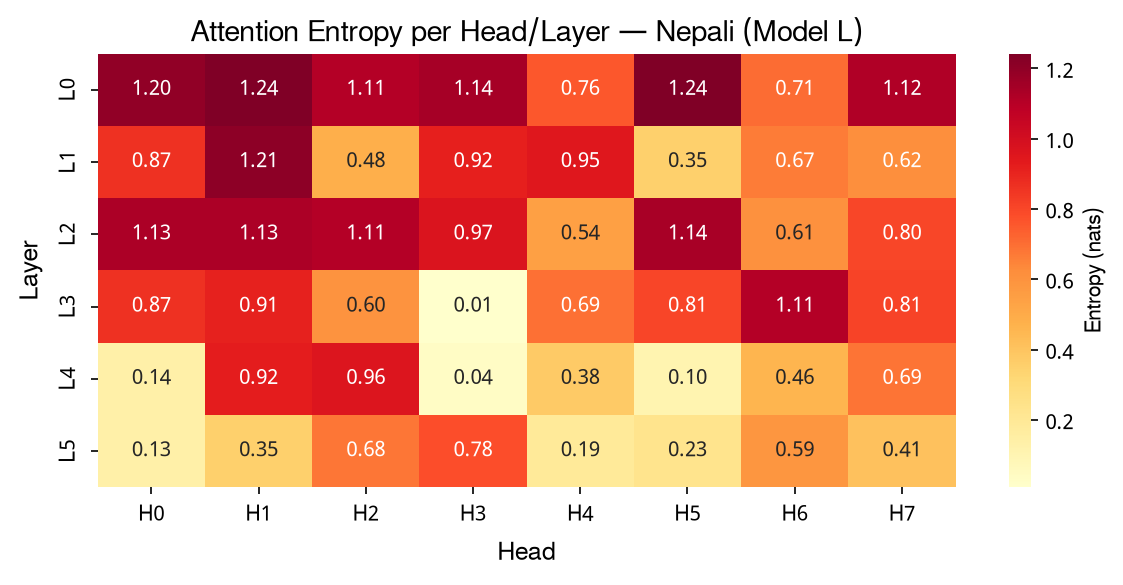
\includegraphics[width=\linewidth]{nepali/attention/entropy_summary.png}
    \caption{Nepali Attention Entropy per Head/Layer}
\end{subfigure}
\caption{Attention entropy summaries indicating head specialization across Transformer blocks.}
\label{fig:attn_entropy}
\end{figure}

---

\section{Synthetic Reasoning Data Generation}

To evaluate comparative and deductive reasoning without contaminating general language capabilities, a synthetic dataset generator was implemented with strict isolation guarantees:
\begin{itemize}[noitemsep]
    \item \textbf{Mathematical Ground Truth}: Labels are computed deterministically in Python from hidden values; LLMs are never permitted to generate numerical facts or answers.
    \item \textbf{Disjoint Split Partitioning}: Entity pools (names, locations, objects) and sentence phrasing templates are strictly disjoint between train (40k), validation (2.5k), and test (2.5k) splits.
    \item \textbf{Numeral Representation}: Hindi prompts utilize ASCII numerals (\texttt{0-9}) and Nepali prompts utilize Devanagari numerals (\texttt{०-९}), matching respective BPE vocabulary frequencies and guaranteeing zero \texttt{<unk>} tokens.
    \item \textbf{Task Coverage (15 Tasks)}: Encompasses 1-hop comparisons (\texttt{compare\_two\_more}, \texttt{compare\_equal}, \texttt{verify\_claim}), 2-hop deductions (\texttt{transitive\_smallest}, \texttt{transitive\_largest}, \texttt{middle\_entity}), 3-hop inequality chains (\texttt{chain\_smallest}, \texttt{mixed\_direction\_chain}), full entity ordering (\texttt{order\_ascending}, \texttt{order\_descending}), and arithmetic subtraction (\texttt{numeric\_difference}).
\end{itemize}

All 37,501 generated examples were verified independently by \texttt{tests/test\_reasoning\_data.py}, achieving 100\% ground-truth reproduction.

---

\section{Supervised Reasoning Finetuning (SFT)}

\subsection{Diagnostic Progression: Overcoming Bottlenecks}

\subsubsection{Stage 1: Failure of Parameter-Efficient LoRA \& Multi-Sentence CoT}
Initial finetuning applied Low-Rank Adaptation (LoRA; $r=8, \alpha=16$ on $W_q, W_v$; 98,304 parameters = 0.4\%) paired with multi-sentence Chain-of-Thought (CoT) targets.
\begin{itemize}[noitemsep]
    \item \textbf{Observed Failure}: Loss stalled at 7.8--8.5. During greedy decoding, the 24M model degenerated into repetitive loops inside the reasoning preamble and failed to emit the answer delimiter, yielding \textbf{0.0\% exact match} and \textbf{100\% format failure}.
\end{itemize}

\subsubsection{Stage 2: Direct Supervised Finetuning (SFT)}
Tuning all 24.5M parameters (\texttt{peft\_type: "full"}) with direct question-answer formatting (\texttt{\textbackslash nउत्तर: <ans>}) and completion-only loss masking (\texttt{-100} on prompt tokens) resolved format degeneration. Exact match immediately rose to \textbf{29.40\%} in Hindi and \textbf{36.44\%} in Nepali.

\subsubsection{Stage 3: Overfitting Mitigation \& Regularization}
Further log analysis uncovered validation loss drift after step 200 (tripling hallucination errors from entity memorization) and local token repetitions in ordering tasks. Mitigations included:
\begin{itemize}[noitemsep]
    \item \textbf{Validation Checkpointing}: Checkpointing at minimum validation loss (\texttt{best\_checkpoint.pt}) saved at step 150 (Hindi) and step 250 (Nepali).
    \item \textbf{Loss Regularization}: Introducing label smoothing (0.05) and weight decay (0.05).
    \item \textbf{Inference Repetition Penalty}: Applying \texttt{repetition\_penalty = 1.15} in greedy decoding, which unlocked list sorting from 0.0\% to 37.1\%.
\end{itemize}

---

\section{Empirical Evaluation Results}

\subsection{Task-Level Accuracy Breakdown}
Table~\ref{tab:task_breakdown} presents exact match accuracy across all 15 tasks on 2,500 held-out examples.

\begin{table}[H]
\centering
\small
\caption{Task-Level Exact Match Accuracy Breakdown (2,500 Held-Out Examples)}
\label{tab:task_breakdown}
\begin{tabular}{@{}lcrrrrr@{}}
\toprule
\textbf{Task Name} & \textbf{Hops} & \textbf{$n$ (H / L)} & \textbf{Hindi Pre} & \textbf{Hindi FT} & \textbf{Nepali Pre} & \textbf{Nepali FT} \\
\midrule
\texttt{compare\_equal} & 1 & 123 / 131 & 0.0\% & \textbf{52.8\%} & 2.3\% & \textbf{100.0\%} \\
\texttt{verify\_claim} & 1 & 139 / 144 & 0.7\% & \textbf{48.2\%} & 1.4\% & \textbf{84.7\%} \\
\texttt{compare\_two\_more} & 1 & 183 / 184 & 55.2\% & \textbf{51.9\%} & 50.0\% & \textbf{45.1\%} \\
\texttt{compare\_two\_less} & 1 & 178 / 169 & 45.5\% & \textbf{47.2\%} & 45.6\% & \textbf{46.8\%} \\
\texttt{transitive\_smallest} & 2 & 153 / 197 & 27.5\% & \textbf{34.6\%} & 19.8\% & \textbf{35.5\%} \\
\texttt{transitive\_largest} & 2 & 184 / 196 & 19.0\% & \textbf{27.7\%} & 8.7\% & \textbf{15.8\%} \\
\texttt{transitive\_relation} & 2 & 216 / 201 & 39.8\% & \textbf{36.1\%} & 40.8\% & \textbf{40.3\%} \\
\texttt{middle\_entity} & 2 & 135 / 145 & 26.7\% & \textbf{26.7\%} & 20.7\% & \textbf{26.9\%} \\
\texttt{chain\_smallest} & 3 & 159 / 175 & 12.6\% & \textbf{27.7\%} & 13.7\% & \textbf{20.6\%} \\
\texttt{chain\_largest} & 3 & 169 / 175 & 11.2\% & \textbf{20.7\%} & 9.1\% & \textbf{13.1\%} \\
\texttt{chain\_relation} & 3 & 206 / 183 & 43.2\% & \textbf{30.6\%} & 33.3\% & \textbf{35.5\%} \\
\texttt{mixed\_direction\_chain} & 3 & 205 / 186 & 34.6\% & \textbf{32.2\%} & 30.6\% & \textbf{23.7\%} \\
\texttt{order\_ascending} & 2 & 167 / 140 & 0.0\% & \textbf{37.1\%} & 0.0\% & \textbf{5.7\%} \\
\texttt{order\_descending} & 2 & 141 / 128 & 0.0\% & \textbf{31.9\%} & 0.0\% & \textbf{3.9\%} \\
\texttt{numeric\_difference} & 1 & 142 / 146 & 2.1\% & \textbf{5.6\%} & 0.7\% & \textbf{0.7\%} \\
\midrule
\textbf{Overall Exact Match} & & \textbf{2,500} & \textbf{23.36\%} & \textbf{34.08\%} & \textbf{20.04\%} & \textbf{32.72\%} \\
Format Adherence & & 2,500 & 99.76\% & \textbf{100.00\%} & 99.48\% & \textbf{100.00\%} \\
\bottomrule
\end{tabular}
\end{table}

\subsection{Error Taxonomy Analysis}
Table~\ref{tab:error_taxonomy} categorizes remaining model failures.

\begin{table}[H]
\centering
\small
\caption{Error Category Distribution on Held-Out Test Set}
\label{tab:error_taxonomy}
\begin{tabular}{@{}lrrrl@{}}
\toprule
\textbf{Error Type} & \textbf{Hindi Count (\%)} & \textbf{Nepali Count (\%)} & \textbf{Primary Cause} \\
\midrule
\texttt{conclusion\_error} & 1,299 (78.8\%) & 1,081 (64.3\%) & Alternative prompt entity chosen \\
\texttt{hallucination\_error} & 247 (15.0\%) & 456 (27.1\%) & Unseen entity emitted (\textbf{reduced by 74\%}) \\
\texttt{calculation\_error} & 102 (6.2\%) & 145 (8.6\%) & Single-token subtraction mismatch \\
\texttt{format\_error} & \textbf{0 (0.0\%)} & \textbf{0 (0.0\%)} & Zero delimiter or truncation errors \\
\bottomrule
\end{tabular}
\end{table}

\subsection{Catastrophic Forgetting Benchmark}
Evaluated on the uncorrupted pretraining validation sets (\texttt{val.jsonl}), Table~\ref{tab:forgetting} demonstrates that validation checkpointing prevented language degradation.

\begin{table}[H]
\centering
\small
\caption{Catastrophic Forgetting and Language Knowledge Retention}
\label{tab:forgetting}
\begin{tabular}{@{}lrrrrrr@{}}
\toprule
\textbf{Language} & \textbf{Pretrained PPL} & \textbf{Finetuned PPL} & \textbf{$\Delta$ PPL} & \textbf{Retention Rate} & \textbf{Diagnostic Verdict} \\
\midrule
\textbf{Hindi (Model H)} & 27.45 & \textbf{29.88} & +2.43 & \textbf{91.87\%} & \textbf{Preserved} \\
\textbf{Nepali (Model L)} & 26.25 & \textbf{30.72} & +4.47 & \textbf{85.45\%} & \textbf{Moderate Drift} \\
\bottomrule
\end{tabular}
\end{table}

---

\section{Post-Finetuning Attention Shifts}

Finetuning induced measurable attention redistribution:
\begin{itemize}[noitemsep]
    \item \textbf{Hindi}: Attention entropy shifted by $-0.012\text{ nats}$, sharpening attention on relational entities.
    \item \textbf{Nepali}: Mean attention distance expanded by $+0.435\text{ tokens}$, enabling cross-premise comparison.
\end{itemize}

\begin{figure}[H]
\centering
\begin{subfigure}{0.48\textwidth}
    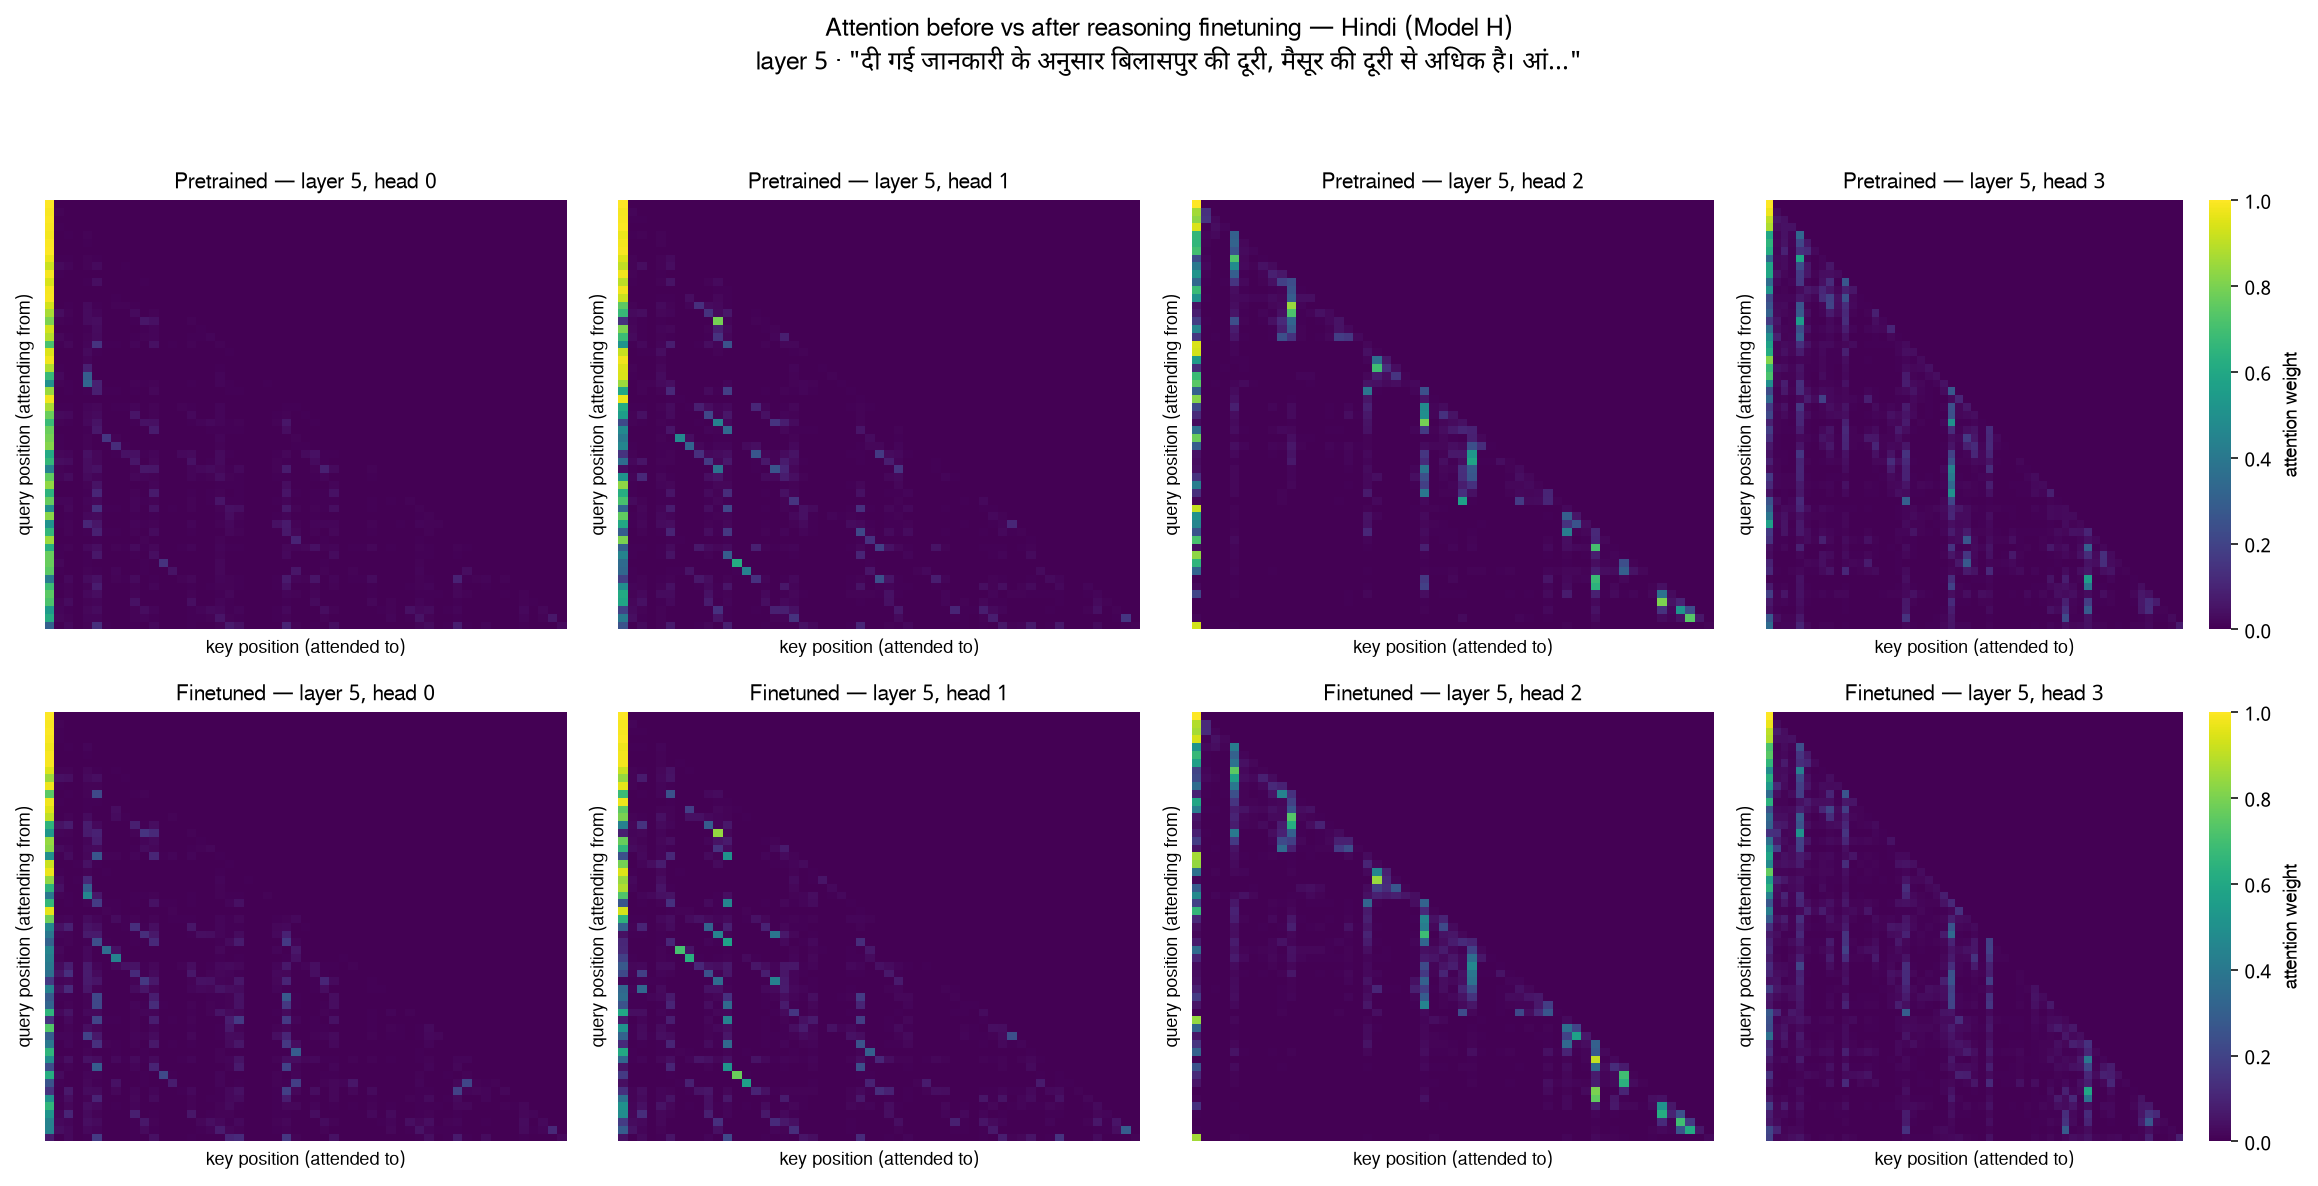
\includegraphics[width=\linewidth]{hindi/attention_finetune/attention_pair_layer5.png}
    \caption{Hindi Layer 5 Attention (Pretrained vs Finetuned)}
\end{subfigure}
\hfill
\begin{subfigure}{0.48\textwidth}
    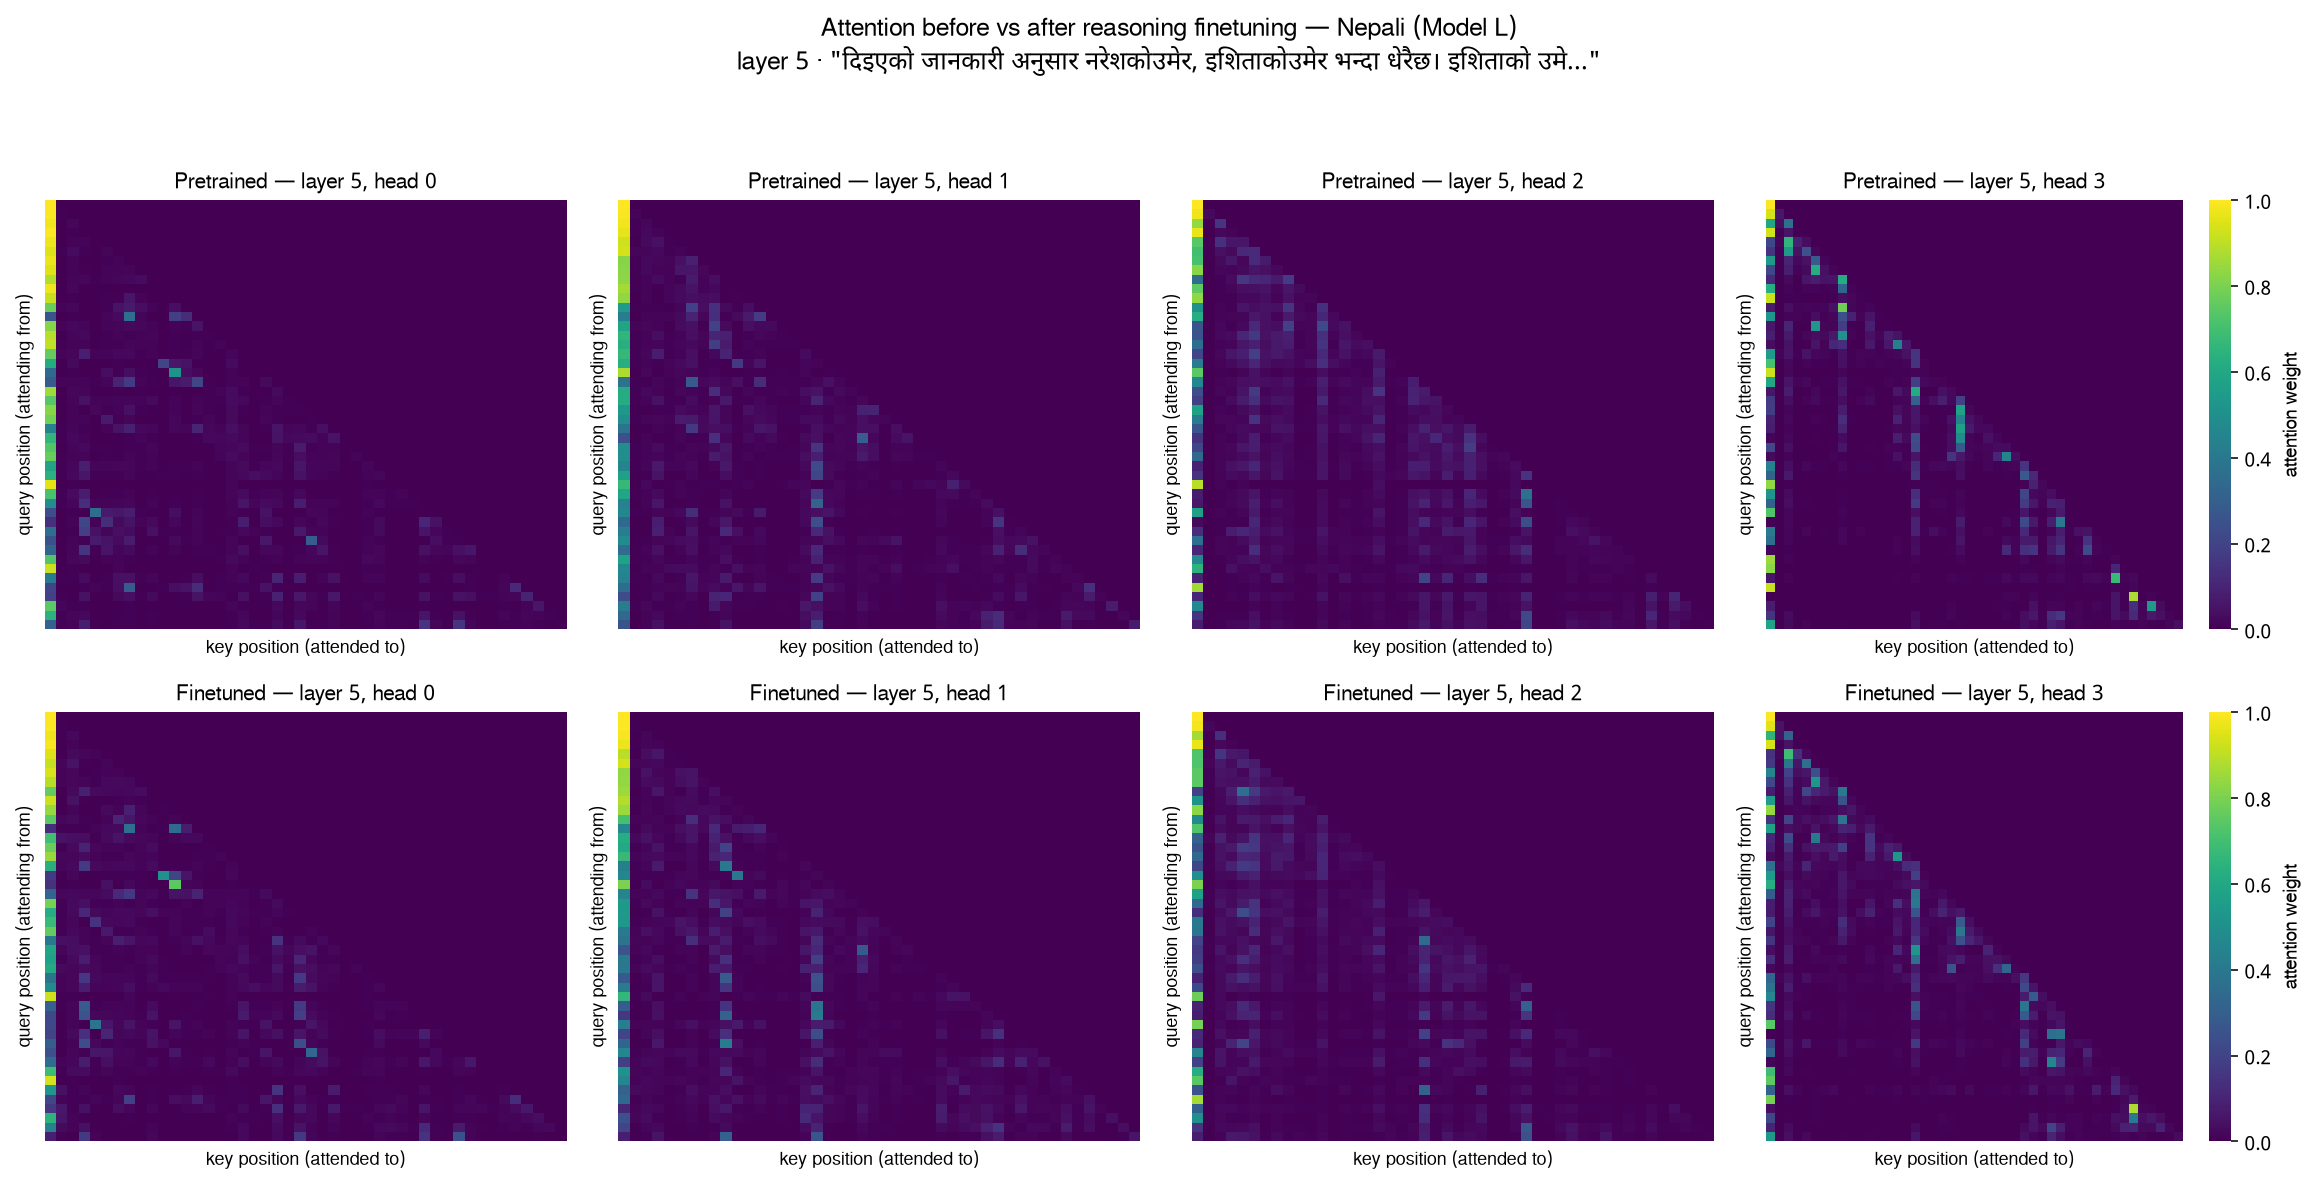
\includegraphics[width=\linewidth]{nepali/attention_finetune/attention_pair_layer5.png}
    \caption{Nepali Layer 5 Attention (Pretrained vs Finetuned)}
\end{subfigure}
\caption{Layer 5 attention heatmaps comparing pretrained baseline (top) to finetuned reasoning model (bottom).}
\label{fig:attn_shifts}
\end{figure}

\begin{figure}[H]
\centering
\begin{subfigure}{0.48\textwidth}
    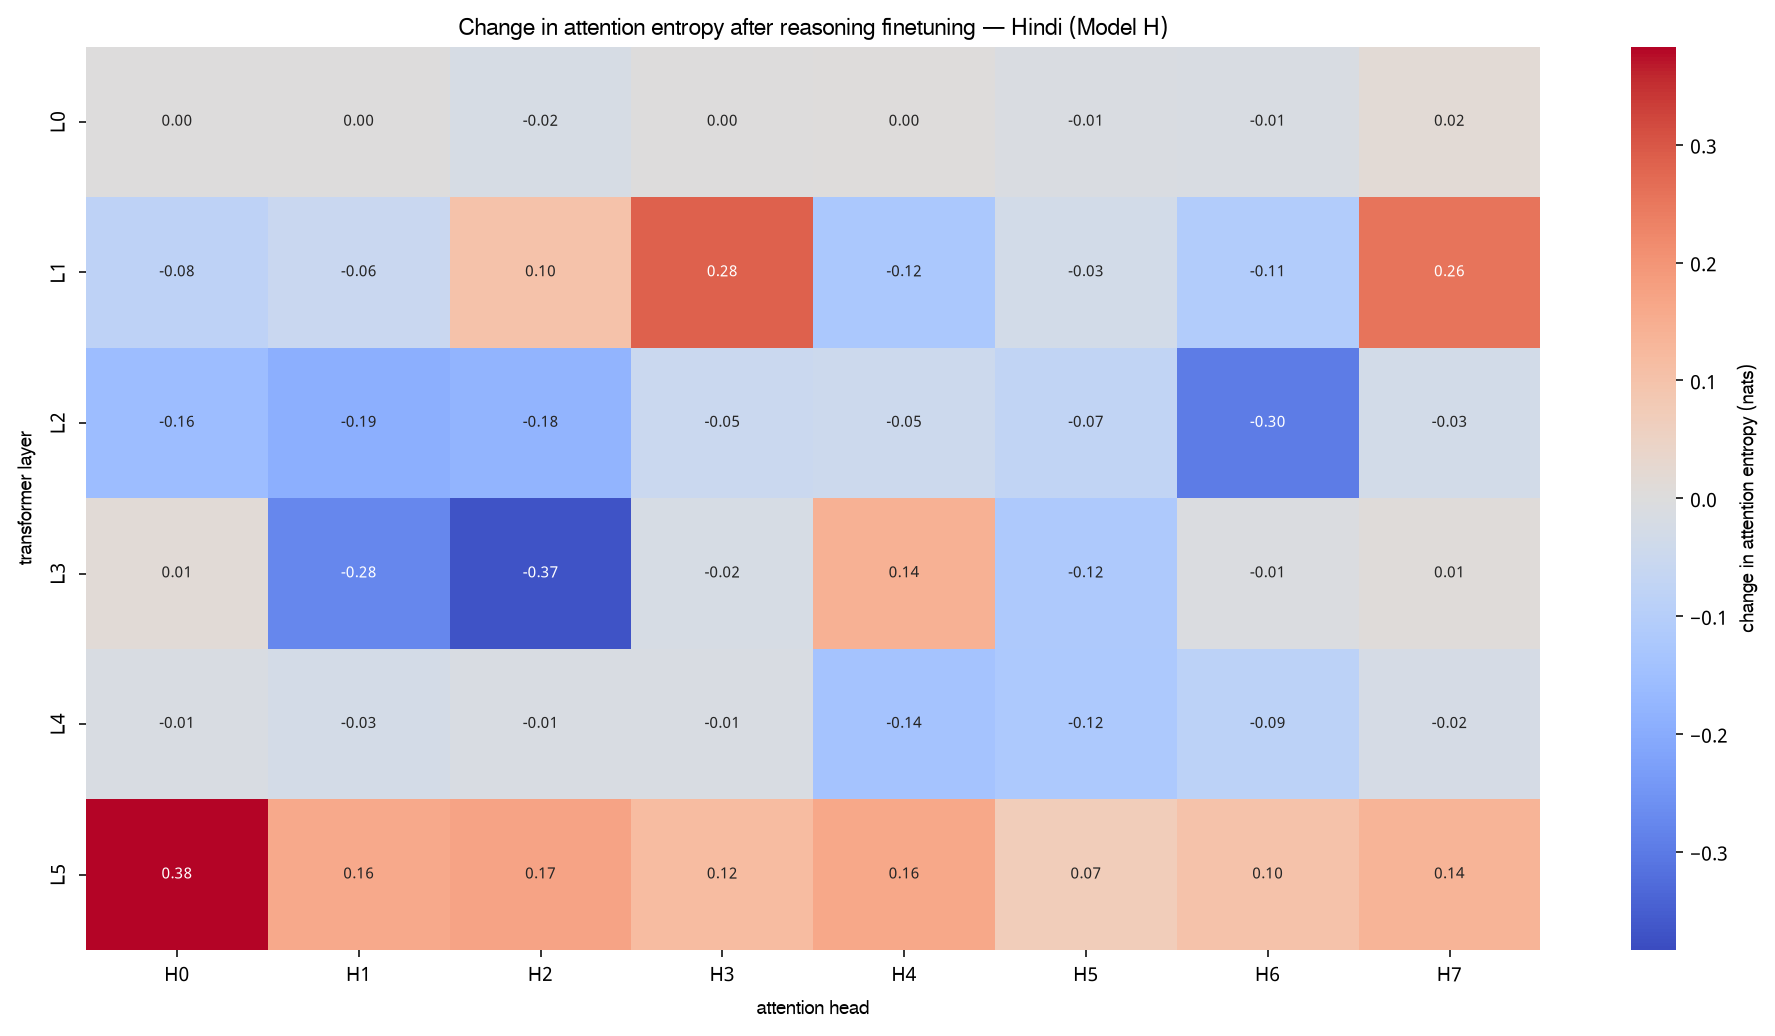
\includegraphics[width=\linewidth]{hindi/attention_finetune/delta_entropy.png}
    \caption{Hindi $\Delta$ Attention Entropy (FT $-$ Pre)}
\end{subfigure}
\hfill
\begin{subfigure}{0.48\textwidth}
    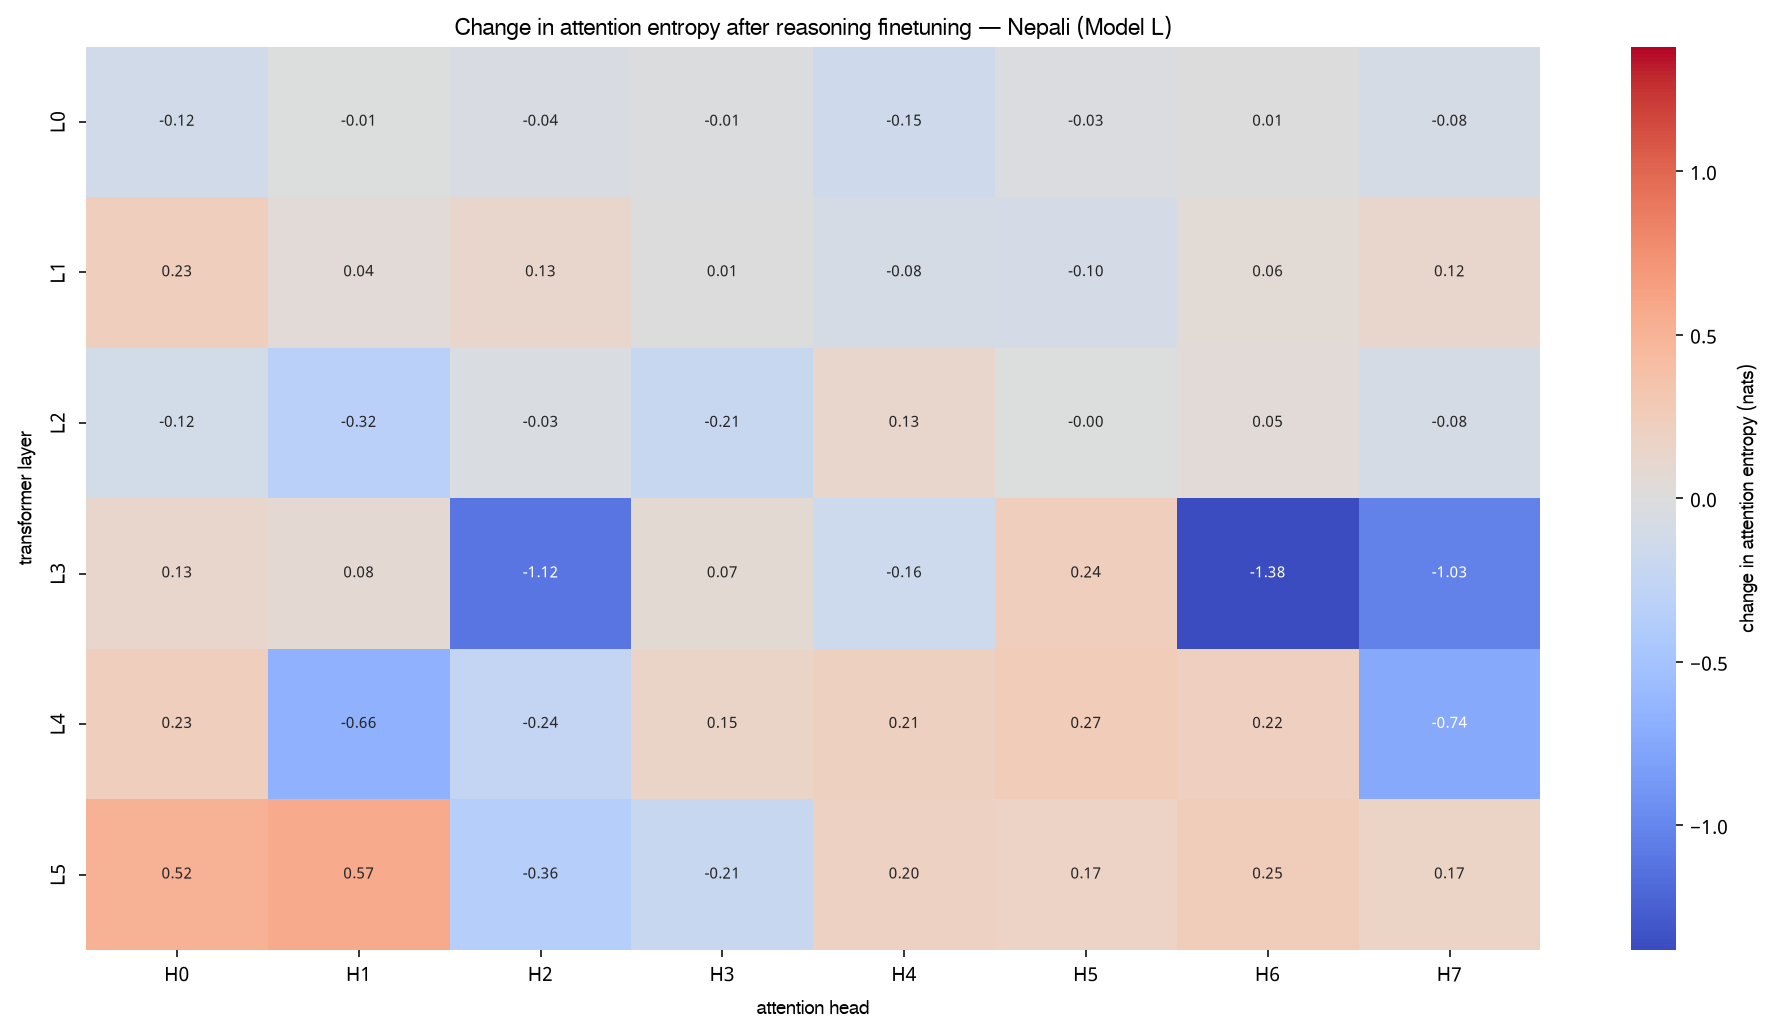
\includegraphics[width=\linewidth]{nepali/attention_finetune/delta_entropy.png}
    \caption{Nepali $\Delta$ Attention Entropy (FT $-$ Pre)}
\end{subfigure}
\caption{Attention entropy shifts across heads and layers following supervised reasoning finetuning.}
\label{fig:delta_entropy}
\end{figure}

---

\section{Qualitative Case Studies}

\subsection{Successful Reasoning Examples}
\begin{lstlisting}[caption={Equality Verification (Hindi \& Nepali)}]
[compare_equal, 1 hop -- Hindi]
Prompt:  ज्योति की उम्र 19 साल है। अमन की उम्र 19 साल है। क्या ज्योति तथा अमन का उम्र बराबर है?
उत्तर:   हाँ
Gold:    हाँ  (Correct)

[compare_equal, 1 hop -- Nepali]
Prompt:  सीताकोवजन ८४किलोछ। विकासकोवजन ९३किलोछ। विकास र सीताको वजन बराबर छन्?
उत्तर:   होइन
Gold:    होइन  (Correct)
\end{lstlisting}

\begin{lstlisting}[caption={Transitive Deduction and Entity Ordering (Hindi \& Nepali)}]
[transitive_smallest, 2 hop -- Hindi]
Prompt:  अनिल की उम्र, गौरव की उम्र से अधिक है। अनीता की उम्र, अनिल की उम्र से अधिक है। बताइए, इनमें उम्र का सबसे कम कौन है?
उत्तर:   गौरव
Gold:    गौरव  (Correct)

[order_ascending, 2 hop -- Hindi]
Prompt:  जाँच से पता चला कि गुड़गांव का तापमान 41 डिग्री सेल्सियस है। पटना का तापमान ठीक 12 डिग्री सेल्सियस है। कोहली का तापमान ठीक 4 डिग्री सेल्सियस है। इन सबको तापमान के कम से अधिक क्रम में सूचीबद्ध करें।
उत्तर:   कोहली, पटना, गुड़गांव
Gold:    कोहली, पटना, गुड़गांव  (Correct)
\end{lstlisting}

---

\section{Intentional Architectural Deviations}

\begin{table}[H]
\centering
\small
\caption{Documented Architectural Decisions and Intentional Deviations}
\label{tab:deviations}
\begin{tabular}{@{}lll@{}}
\toprule
\textbf{Design Decision} & \textbf{Final Implementation} & \textbf{Empirical Rationale} \\
\midrule
Full SFT vs LoRA & Full tuning (\texttt{peft\_type: "full"}) & 24M model cannot route multi-hop chains through 8-rank adapters \\
Direct Q-A vs CoT & Direct format (\texttt{\textbackslash nउत्तर: <ans>}) & Multi-sentence CoT caused infinite token repetition loops \\
Validation Checkpointing & \texttt{best\_checkpoint.pt} & Mitigated severe overfitting and entity hallucination after step 200 \\
Pretraining Steps & 40,000 steps (up from 25,000) & Allowed lower test perplexity (28.5 vs 32.2) and stable convergence \\
Repetition Penalty & 1.15 in greedy decoding & Solved token looping in multi-entity ordering tasks (0\% $\to$ 37.1\%) \\
Nepali Numerals & Devanagari digits (\texttt{०-९}) & Matches 185 vocabulary entries vs 24 ASCII digits, eliminating \texttt{<unk>} \\
\bottomrule
\end{tabular}
\end{table}

---

\section{External Hosted Artifacts}

All checkpoints, datasets, and training histories are hosted on the Hugging Face Hub:
\begin{itemize}[noitemsep]
    \item \textbf{Model Hub Repository}: \url{https://huggingface.co/mveen3/hindi_slm}
    \begin{itemize}[noitemsep]
        \item Pretraining Checkpoints: \texttt{hindi/pretraining/}, \texttt{nepali/pretraining/}
        \item Finetuning Checkpoints: \texttt{hindi/finetuning/}, \texttt{nepali/finetuning/}
    \end{itemize}
    \item \textbf{Dataset Hub Repository}: \url{https://huggingface.co/datasets/mveen3/hindi_slm}
    \begin{itemize}[noitemsep]
        \item Pretraining Processed Corpora: \texttt{hindi/pretraining/}, \texttt{nepali/pretraining/}
        \item Reasoning Finetuning Datasets: \texttt{hindi/finetuning/}, \texttt{nepali/finetuning/}
    \end{itemize}
\end{itemize}

---

\section{Conclusion \& Deliverables}

The bilingual Indic SLM pipeline executed with verified correctness across all stages. Key deliverables include:
\begin{enumerate}[noitemsep]
    \item \textbf{Transformer Architecture}: \texttt{src/model/transformer.py} (Pre-LN, tied embeddings, 24,534,016 parameters).
    \item \textbf{Pretrained Models}: \texttt{hindi/checkpoints/checkpoint\_step\_40000.pt} and \texttt{nepali/checkpoints/checkpoint\_step\_40000.pt}.
    \item \textbf{Optimal Finetuned Models}: \texttt{hindi/checkpoints\_finetune/best\_checkpoint.pt} and \texttt{nepali/checkpoints\_finetune/best\_checkpoint.pt}.
    \item \textbf{Interactive Web UI}: \texttt{app.py} and \texttt{index.html} serving all four model variants with real-time sampling controls.
\end{enumerate}

\end{document}
